%This Template was created by Stephen Myall 20th April 2018



%----------------------------------------------------------------------------------------
%	PACKAGES AND OTHER DOCUMENT CONFIGURATIONS **(DO NOT CHANGE)**
%----------------------------------------------------------------------------------------
\documentclass[a4paper,10pt]{article}

\usepackage[english]{babel}
\usepackage[T1]{fontenc}
\usepackage[utf8]{inputenc}
\usepackage[scaled=0.95]{helvet}
\renewcommand{\familydefault}{\sfdefault}
\usepackage{lmodern}
\usepackage{lipsum} % Required to insert dummy text. To be removed otherwise
\usepackage{xcolor}
\usepackage{titlesec}
\usepackage{parskip}
\usepackage{fancyhdr}
\usepackage{hyperref}
\usepackage{lastpage}
\usepackage{tocloft}
\usepackage{enumitem}
\usepackage[most]{tcolorbox}
    
    % Use to add letters or roman numerals to lists  
    % \begin{enumerate}[label=(\alph*)]
    % \begin{enumerate}[label=(\roman*)]
%----------------------------------------------------------------------------------------
%	COLOURS - **(DO NOT CHANGE)**
%----------------------------------------------------------------------------------------

\definecolor{color1}{RGB}{0,0,90} % Color of the article title and sections
\definecolor{color2}{RGB}{0,20,20}

%----------------------------------------------------------------------------------------
%	HYPERLINKS - **(DO NOT CHANGE)**
%----------------------------------------------------------------------------------------

\usepackage{hyperref} % Required for hyperlinks
\hypersetup{hidelinks,colorlinks,breaklinks=true,urlcolor=color2,citecolor=color1,linkcolor=color1,bookmarksopen=false,pdftitle={Title},pdfauthor={Author}}

%----------------------------------------------------------------------------------------
%	Adds a colour block behind section title - **(DO NOT CHANGE)**
%----------------------------------------------------------------------------------------

\titleformat{name=\section}[block]
  {\sffamily\huge}
  {}
  {0pt}
  {\colorsection}
\titlespacing*{\section}{0pt}{\baselineskip}{\baselineskip}

\newcommand{\colorsection}[1]{%
  \colorbox{blue!20}{\parbox{\dimexpr\textwidth-2\fboxsep}{\thesection\ #1}}}

%If you want white on colored text, just modify the \colorsection command, for example as
%\newcommand{\colorsection}[1]{%
 % \colorbox{blue}{\parbox{\dimexpr\textwidth-2\fboxsep}{\color{white}\thesection\ #1}}}
 
%----------------------------------------------------------------------------------------
%	Sets the Page Margins - **(DO NOT CHANGE)**
%----------------------------------------------------------------------------------------
 
\usepackage{vmargin}
\setmarginsrb{2.5 cm}{1.5 cm}{1 cm}{1.5 cm}{1 cm}{1.5 cm}{1 cm}{1.5 cm}

%----------------------------------------------------------------------------------------
%	Needed to Add Images **(DO NOT CHANGE)**
%----------------------------------------------------------------------------------------

\usepackage{graphicx}
\graphicspath{{images/}}

%----------------------------------------------------------------------------------------
%	Removes Default Hyphenation  **(DO NOT CHANGE)**
%----------------------------------------------------------------------------------------
\tolerance=1
\emergencystretch=\maxdimen
\hyphenpenalty=10000
\hbadness=10000

%----------------------------------------------------------------------------------------
%	Enter the Title and Author here
%----------------------------------------------------------------------------------------

\title{Document Management Template}
\author{Stephen Myall}
\date{}

\makeatletter
\let\runtitle\@title
\let\theauthor\@author
\let\thedate\@date
\makeatother

%----------------------------------------------------------------------------------------
%	Flowcharts - **(DO NOT CHANGE)**
%----------------------------------------------------------------------------------------

\usepackage{verbatim}
\usepackage{tikz}
\usetikzlibrary{arrows.meta}
\tikzset{%
  >={Latex[width=2mm,length=2mm]},
  % Specifications for style of nodes:
            base/.style = {rectangle, rounded corners, draw=black,
                           minimum width=4cm, minimum height=1cm,
                           text centered, font=\sffamily},
  activityStarts/.style = {base, fill=blue!30},
       startstop/.style = {base, fill=red!30},
    activityRuns/.style = {base, fill=green!30},
         process/.style = {base, minimum width=2.5cm, fill=orange!15,
                           font=\ttfamily},
}


%----------------------------------------------------------------------------------------
%	Header and Footer Configuration - **(DO NOT CHANGE)**
%----------------------------------------------------------------------------------------

\pagestyle{fancy}
\fancyhf{}
%----------------------------------------------------------------------------------------
%Header - **(DO NOT CHANGE)**
%----------------------------------------------------------------------------------------
\lhead{\runtitle}
\rhead{Page \thepage\ of \pageref{LastPage}}
\renewcommand{\footrulewidth}{0.4pt}% default is 0pt

%----------------------------------------------------------------------------------------
%Footer - **(DO NOT CHANGE)**
%----------------------------------------------------------------------------------------
\lfoot  {Northside Partnership - Internal}
\rfoot{\scriptsize \textit{Note: Revisions to this document may have been issued since it was printed}}

%----------------------------------------------------------------------------------------
%	This is the Beginning of the Document - **(DO NOT CHANGE)**
%----------------------------------------------------------------------------------------

\begin{document}

%----------------------------------------------------------------------------------------
%	This is the Title Page
%----------------------------------------------------------------------------------------

\begin{titlepage}
	
	\centering
	    

        \vspace*{0.5 cm}
%----------------------------------------------------------------------------------------
%	This is the Logo on the Title Page
%----------------------------------------------------------------------------------------       
        
            \includegraphics[scale = 0.35]{logo.png}\\[1.0 cm]
    
%----------------------------------------------------------------------------------------
%	This is `the company name' | Document Title, ID and Type
%----------------------------------------------------------------------------------------             
            
            {\LARGE Northside Partnership}\\ % Company Name
            
            \vspace*{1.5 cm}
	
	        \rule{\linewidth}{0.2 mm} \\[0.4 cm]
	        { \Huge \bfseries \runtitle}\\
	         \vspace*{0.5 cm}
	        { \Large \bfseries This is a subtitle}\\
	        \rule{\linewidth}{0.2 mm} \\[1.5 cm]
	        
	          \vspace*{2.5 cm}

            {\huge Standard Operation Procedure}\\[0.5 cm]	% This is the Document Type 
	        
	        \vspace*{4.0 cm}
	   

%----------------------------------------------------------------------------------------
%	This is the Table at the bottom of the title page
%----------------------------------------------------------------------------------------	

  \begin{tabular}{ |l c r |}                                       \hline
    
    Document ID         & \hspace*{4.5 cm}  &   NSP-SOP-IM-001   \\ \hline
    
    Revision Number     & \hspace*{4.5 cm}  &   1.0             \\ \hline
    
    Document Author     & \hspace*{4.5 cm}  &   Stephen Myall   \\ \hline
    
    Document Status     & \hspace*{4.5 cm}  &   Draft           \\ \hline
    
    Last Updated        & \hspace*{4.5 cm}  &   17th June 2018  \\ \hline
    
    Date Printed        & \hspace*{4.5 cm}  &   \today          \\ \hline
   
   \end{tabular}

  \end{titlepage} 
	
%----------------------------------------------------------------------------------------
%	This is the Table of Contents - **(DO NOT CHANGE)**
%----------------------------------------------------------------------------------------


\tableofcontents %Displays Table of Contents
\thispagestyle{empty}  %Removes header and footer
\pagebreak %Starts new page after table of contents
\setcounter{page}{1} %Starts the new page counter to 1

%----------------------------------------------------------------------------------------
%	This is where the actual content begins
%----------------------------------------------------------------------------------------

\section{Title of my first section}
    
\subsection{Title of my first subsection}
 \subsection{Title of my second subsection}
    
    \subsubsection{Ordered list using letters} 
        \begin{enumerate}[label=(\alph*)]
            \item First item on list
            \item Second item on list
            \item Third item on list
        \end{enumerate}
        
    \subsubsection{Ordered list using roman numerals} 
      \begin{enumerate}[label=(\roman*)]
            \item First item on list
            \item Second item on list
            \item Third item on list
        \end{enumerate}
        
     \subsubsection{Unordered List - Bullets} 
      \begin{itemize}
            \item First item on list
            \item Second item on list
            \item Third item on list
        \end{itemize}     
    
 
\section{Title of my second section - \textit{Paragragh Text Sample}}
        \lipsum

\subsection{This displays a scaleable Image}

    \subsubsection{Image scaled to 25 percent of its original size}            
            
            \begin{center}
                \includegraphics[scale = 0.25]{logo.png}\\[1.0 cm]
            \end{center}
                \subsubsection{Same image scaled to 50 percent of its original size} 
            
           \begin{center}
                \includegraphics[scale = 0.50]{logo.png}\\[1.0 cm]
            \end{center}
    

 \subsection{A two column table spanning page width}
            
            \begin{center}
                 \vspace*{0.5 cm}
                
        \begin{tabular}{|  p{3.5cm}  |  p{13cm} |}
        
                                       \hline
\textbf{Document ID} & \textbf{Document Title}\\  \hline
NSP-POL-QA    & NSP Quality Policy    \\ \hline
NSP-POL-HR    & NSP Human Resource Policy  \\ \hline
NSP-POL-IM    & NSP Information Management Policy   \\ \hline
NSP-POL-FIN   & NSP Finance Policy  \\ \hline
NSP-POL-HS    & NSP Health and Safety Policy  \\ \hline

        \end{tabular}
    \vspace*{1 cm}
\end{center}

\section{Example of Workflow}
\subsection{Process for XXXXXXX XXXXXX}
% Drawing part, node distance is 1.5 cm and every node
% is prefilled with white background
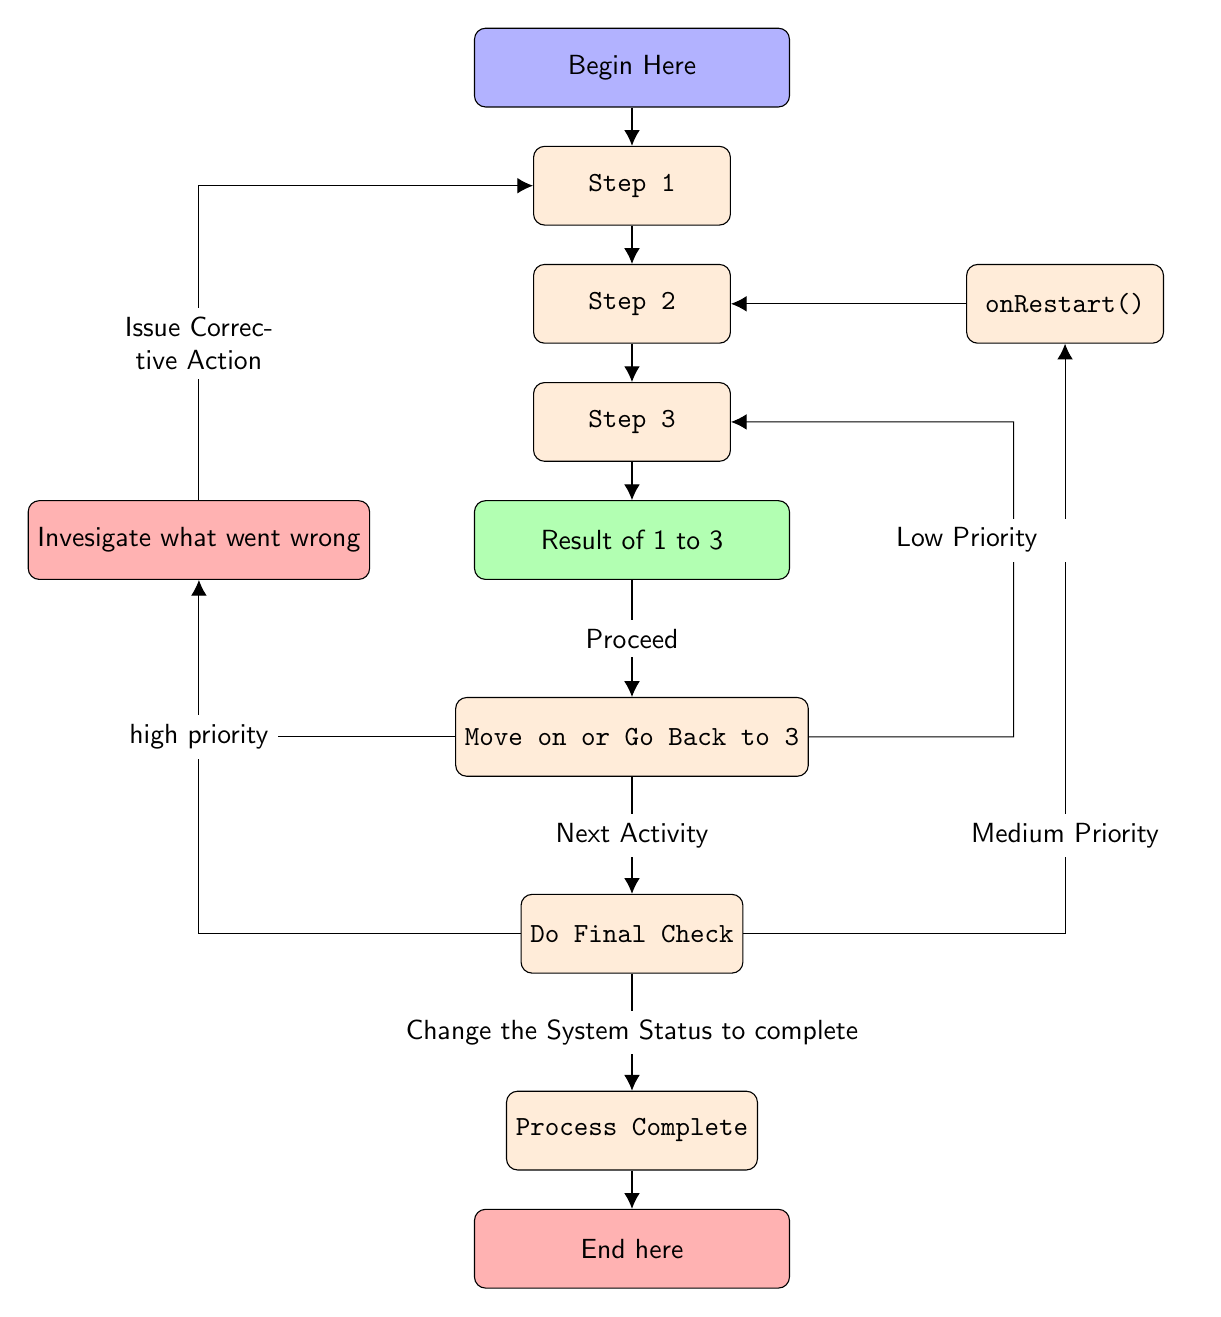
\begin{tikzpicture}[node distance=1.5cm,
    every node/.style={fill=white, font=\sffamily}, align=center]
  % Specification of nodes (position, etc.)
  \node (start)             [activityStarts]              {Begin Here};
  \node (onCreateBlock)     [process, below of=start]          {Step 1};
  \node (onStartBlock)      [process, below of=onCreateBlock]   {Step 2};
  \node (onResumeBlock)     [process, below of=onStartBlock]   {Step 3};
  \node (activityRuns)      [activityRuns, below of=onResumeBlock]
                                                      {Result of 1 to 3};
  \node (onPauseBlock)      [process, below of=activityRuns, yshift=-1cm]
                                                                {Move on or Go Back to 3};
  \node (onStopBlock)       [process, below of=onPauseBlock, yshift=-1cm]
                                                                 {Do Final Check};
  \node (onDestroyBlock)    [process, below of=onStopBlock, yshift=-1cm] 
                                                              {Process Complete};
  \node (onRestartBlock)    [process, right of=onStartBlock, xshift=4cm]
                                                              {onRestart()};
  \node (ActivityEnds)      [startstop, left of=activityRuns, xshift=-4cm]
                                                        {Invesigate what went wrong};
  \node (ActivityDestroyed) [startstop, below of=onDestroyBlock]
                                                    {End here};     
 
 
  % Specification of lines between nodes specified above
  % with aditional nodes for description 
  \draw[->]             (start) -- (onCreateBlock);
  \draw[->]     (onCreateBlock) -- (onStartBlock);
  \draw[->]      (onStartBlock) -- (onResumeBlock);
  \draw[->]     (onResumeBlock) -- (activityRuns);
  \draw[->]      (activityRuns) -- node[text width=4cm]
                                   {Proceed} (onPauseBlock);
  \draw[->]      (onPauseBlock) -- node {Next Activity}
                                   (onStopBlock);
  \draw[->]       (onStopBlock) -- node {Change the System Status to complete} (onDestroyBlock);
  \draw[->]    (onRestartBlock) -- (onStartBlock);
  \draw[->]       (onStopBlock) -| node[yshift=1.25cm, text width=3cm]
                                   {Medium Priority}
                                   (onRestartBlock);
  \draw[->]    (onDestroyBlock) -- (ActivityDestroyed);
  \draw[->]      (onPauseBlock) -| node(priorityXMemory)
                                   {high priority}
                                   (ActivityEnds);
  \draw           (onStopBlock) -| (priorityXMemory);
  \draw[->]     (ActivityEnds)  |- node [yshift=-2cm, text width=3.1cm]
                                    {Issue Corrective Action}
                                    (onCreateBlock);
  \draw[->] (onPauseBlock.east) -- ++(2.6,0) -- ++(0,2) -- ++(0,2) --                
     node[xshift=1.2cm,yshift=-1.5cm, text width=2.5cm]
     {Low Priority}(onResumeBlock.east);
  \end{tikzpicture}
  
  \subsection{Process Clarification Points}
          \begin{enumerate}[label=(\alph*)]
            \item First item on list
            \item Second item on list
            \item Third item on list
        \end{enumerate}
 \newpage 
\section{Using Colour Boxes}

\begin{tcolorbox}[colback=blue!5!white,colframe=blue!75!black,title=Colour Box title]
  You can put anything you want in here
\end{tcolorbox}
%----------------------------------------------------------------------------------------
%	This is the End of the Document
%----------------------------------------------------------------------------------------
\end{document}
